
\chapter{Non-Conforming Methods for the Plate Problem}\label{chap11}

WE\pageoriginale START WITH a brief classification of finite element
methods. The first class of methods are called {\em conforming
  methods}, which we have described upto now, except when we
considered numerical integration. The second class consists of methods
other than conforming. In the latter class we have the {\em
  Non-conforming} methods included:

Given the abstract problem, the {\em conforming methods} deal with the
finding of subspaces $V_{h}\subset V$ and solving the problems
\begin{equation*}
a_{h}(u_{h},v_{h})=f_{h}(v_{h}),\quad\text{for all}\quad v_{h}\in
V_{h},\tag*{$(P_{h})$} 
\end{equation*}
where $a_{h}=a$ and $f_{h}=f$ for all $h$ and $u_{h}\in V_{h}$ is the
required solution.

When we employ methods other than conforming we commit, in the
terminology of G.\@ Strang, ``Variational Crimes''. (See Strang and
Fix \cite{key22}). These may occur in the following ways:
\begin{itemize}
\item[(i)] When performing numerical integration, we may have $a_{h}$
  and $f_{h}$ different from $a$ and $f$ respectively. However,
  $V_{h}$ is a subspace of $V$;

\item[(ii)] The boundary $\Gamma$ of $\Omega$ may be curved. In this
  case triangles lying in the interior will be triangles of straight
  edges while those meeting the boundary will have curved edges like
  parabolas. These are the so-called ``isoparametric'' finite
  elements. Hence if $\Omega_{h}$ is the union of the finite elements
  of the triangulation $\mathfrak{t}_{h}$, then, in general,
  $\Omega_{h}\neq \Omega$ and consequently $V_{h}\not\subset V$ (where
  $V_{h}$ is a space of functions defined over $\Omega_{h}$),
  $a_{h}\neq a$, $f_{h}\neq f$; for a discussion of these, see Ciarlet
  and Raviart \cite{key30}, \cite{key31}.

\item[(iii)] When employing {\em non-conforming methods} (which will
  be dealt with subsequently) though $\Omega_{h}=\Omega$, $f_{h}=f$,
  we will have $V_{h}\not\subset V$ and $a_{h}\neq a$.

\item[(iv)] One\pageoriginale may employ any combination of the above three.
\end{itemize}

Let us return to the plate problem. For a conforming method we need
the inclusion $V_{h}\subset H^{2}_{0}(\Omega)$ which essentially
results from the inclusion $V_{h}\subset
C^{1}(\overline{\Omega})$. Because of this necessity, when compared
with second-order problems, we either have the dimension of $P_{K}$
``large'' (as in the case of the Argyris triangle) or that the
structure of $P_{K}$ is complicated (as in the HCT-triangle). Also one
would like to have just $P_{K}=P_{2}$ since $u$ is only in
$H^{3}(\Omega)$ in most cases, but this is impossible by the
\v{Z}eni\v{s}ek result (cf.\@ Remark~\ref{chap4-rem4.3}) which
stresses that at least polynomials of degree 5 must be present in
$P_{K}$.

Hence the desire to surmount these difficulties led to the devising of
non-conforming methods, essentially developed by the Engineers.

Since the root of all trouble is the inclusion $V_{h}\subset
H^{2}_{0}(\Omega)$, we drop this condition. Thus we start with
$V_{h}\subset C^{0}(\overline{\Omega})$ and it is much easier from the
computer programme view point. This of course, works only for a few
finite elements, and we describe one of them.

\begin{example}\label{chap11-exam11.1}
The Adini's rectangle; cf.\@ Fig.~\ref{chap11-fig11.1}.
\begin{figure}[H]
\centering
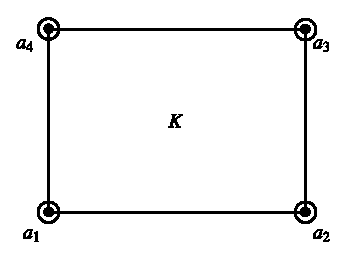
\includegraphics{figure/fig11.1.eps}
\caption{}\label{chap11-fig11.1}
\end{figure}

The element $K$ consists of a rectangle with vertices $\{a_{i},1\leq
i\leq 4\}$; the space $P_{K}$ is given by $P_{K}=P_{3}\oplus
\{x_{1}x^{3}_{2}\}\oplus \{x^{3}_{1}x_{2}\}$, by which we mean
polynomials of degree $\leq 4$ whose only fourth-degree terms are
those involving $x_{1}x^{3}_{2}$ and $x^{3}_{1}x_{2}$. Thus
$P_{3}\subset P_{K}$. We have the set of degrees of freedom:
$$
\sum_{K}=\left\{p(a_{i}),\frac{\p p}{\p x_{1}}(a_{i}),\ \frac{\p p}{\p
  x_{2}}(a_{i}),\ 1\leq i\leq 4\right\}.
$$\pageoriginale

Of course this element can be used only for plates with sides parallel
to the coordinate axes, such as rectangular plates.
\end{example}

\begin{exercise}\label{chap11-exer11.1}
Show that in Example \ref{chap11-exam11.1}, $\sum_{K}$ is
$P_{K}$-unisolvent and that Adini's rectangle is a finite element of
class $C^{0}$, and, in general, not of class $C^{1}$.
\end{exercise}

Thus we get `a priori' that $V_{h}\subset H^{1}(\Omega)$. For the
boundary condition, we set all degrees of freedom on the boundary
nodes as zero. This gives us that $V_{h}\subset
H^{1}_{0}(\Omega)$. Thus the only `unknown' or `free' parameters are
the degrees of freedom at the interior nodes. Note that $\dfrac{\p
  v_{h}}{\p \nu}$ is zero only at the boundary nodes, in general.

In the abstract problem, we have $a(\cdot,\cdot)$ and $f(\cdot)$ given
by
{\fontsize{10}{12}\selectfont
\begin{equation*}
\begin{cases}
a(u,v)=\int\limits_{\Omega}\left[\Delta u\Delta
  v+(1-\sigma)\left(2\dfrac{\p^{2}u}{\p x_{1}\p x_{2}}\dfrac{\p^{2}v}{\p
    x_{1}\p x_{2}}-\dfrac{\p^{2}u}{\p x^{2}_{1}}\dfrac{\p^{2}v}{\p
    x^{2}_{2}}-\dfrac{\p^{2}u}{\p x^{2}_{2}}\dfrac{\p^{2}v}{\p
    x^{2}_{1}}\right)\right]dx,\\ 
f(v)=\int\limits_{\Omega}fvdx,\ f\in L^{2}(\Omega).
\end{cases}\tag{11.1}\label{chap11-eq11.1}
\end{equation*}}

The second integral is defined over $V_{h}$ as well. Thus for the
discrete problem $(P_{h})$ we may set $f_{h}=f$. However while for
$u$, $v\in V_{h}$ the first integral is defined over each
$K\in\mathfrak{t}_{h}$, we cannot define it over $\Omega$, since we
get Dirac measure-like terms along the boundary. To get over this, we
now define
{\fontsize{9}{11}\selectfont
\begin{equation*}
\begin{split}
& a_{h}(u_{h},v_{h})=\sum\limits_{K\in\mathfrak{t}_{h}}\int\limits_{K}\left[\Delta
  u_{h}\Delta v_{h}+(1-\sigma)\left(2\frac{\p^{2}u_{h}}{\p x_{1}\p
    x_{2}}\frac{\p^{2}v_{h}}{\p x_{1}\p x_{2}}-\frac{\p^{2}u_{h}}{\p
    x^{2}_{1}}-\frac{\p^{2}u_{h}}{\p x^{2}_{2}}\frac{\p^{2}v_{h}}{\p
    x^{2}_{1}}\right)\right]dx\\ 
& =\sum\limits_{K\in\mathfrak{t}_{h}}\int\limits_{K}\left[\sigma\Delta
    u_{h}\Delta v_{h}+(1-\sigma)\left(\frac{\p^{2}u_{h}}{\p
      x^{2}_{1}}\frac{\p^{2}v_{h}}{\p x^{2}_{1}}+\frac{\p^{2}u_{h}}{\p
      x^{2}_{2}}\frac{\p^{2}v_{h}}{\p
      x^{2}_{2}}+2\frac{\p^{2}u_{h}}{\p x_{1}\p
      x_{2}}\frac{\p^{2}v_{h}}{\p x_{1}\p x_{2}}\right)\right]dx,
\end{split}\tag{11.2}\label{chap11-eq11.2}
\end{equation*}}
and we have the discrete problem $(P_{h})$: To find $u_{h}\in V_{h}$
such that for all $v_{h}\in V_{h}$ 
\begin{equation*}
a_{h}(u_{h},v_{h})=f(v_{h}).\tag{11.3}\label{chap11-eq11.3}
\end{equation*}\pageoriginale

We now prove the existence and uniqueness of the solution $u_{h}$ for
$(P_{h})$. We define on $V_{h}$ the seminorm
\begin{equation*}
||v_{h}||_{h}=\left(\sum_{K\in\mathfrak{t}_{h}}|v_{h}|^{2}_{2,K}|^{2}_{2,K}\right)^{\frac{1}{2}}. \tag{11.4}\label{chap11-eq11.4}
\end{equation*}

Notice that this may be defined over $V=H^{2}_{0}(\Omega)$ as well and
for $v\in V$, $||v||_{h}=|v|_{2,\Omega}$. In the same way for $u$,
$v\in V$, $a_{h}(u,v)=a(u,v)$.

We now show that the {\em seminorm} $||\cdot||_{h}$ {\em is indeed a
  norm} on $V_{h}$. Let $v_{h}\in V_{h}$ with $||v_{h}||_{h}=0$. This
gives that $\dfrac{\p v_{h}}{\p x_{1}}=$ constant over any $K$. But
given adjacent finite elements the value of $\dfrac{\p v_{h}}{\p
  x_{1}}$ at the common vertices coincide and hence $\dfrac{\p
  v_{h}}{\p x_{1}}$ is constant over $\overline{\Omega}$. But this is
zero on the boundary nodes. Hence $\dfrac{\p v_{h}}{\p x_{1}}=0$ on
$\overline{\Omega}$. Similarly $\dfrac{\p v_{h}}{\p x_{2}}=0$ on
$\overline{\Omega}$. Since $V_{h}\subset C^{0}(\Omega)$ and $v_{h}=0$
on $\Gamma$, the above conditions give that $v_{h}=0$ over
$\overline{\Omega}$. Thus \eqref{chap11-eq11.4} defines a norm on
$V_{h}$.

To show the existence and uniqueness of the solution of $(P_{h})$, we
show that $a_{h}(\cdot,\cdot)$ is $V_{h}$-elliptic. In fact we do more
than this. We show that the $a_{h}(\cdot,\cdot)$ are $V_{h}$-elliptic
uniformly with respect to $h$.

Recall that from physical considerations, $0<\sigma <\frac{1}{2}$ (see
Sec.~\ref{chap2}). Now
\begin{equation*}
\begin{split}
a(v_{h},v_{h}) &=
\sum_{K\in\mathfrak{t}_{h}}\int\limits_{K}\sigma(\Delta
v_{h})^{2}dx+(1-\sigma)||v_{h}||^{2}_{h}\\
&\geq (1-\sigma)||v_{h}||^{2}_{h}.
\end{split}\tag{11.5}\label{chap11-eq11.5}
\end{equation*}

\begin{remark}\label{chap11-rem11.1}
It was mentioned in passing in Sec.~\ref{chap10} that in order to
apply non-conforming methods one needed the second term involving
$\sigma$ in the integral defining $a(\cdot,\cdot)$. The uniform
$V_{h}$-ellipticity could not be got in the Hydrodynamical case where
this term is absent.
\end{remark}

We\pageoriginale now proceed with the abstract error analysis.

\begin{theorem}[STRANG]\label{chap11-thm11.1}
Let $a_{h}(\cdot,\cdot)$ be $V_{h}$-elliptic uniformly with respect to
$h$ with $\widetilde{\alpha}>0$ so that for all $v_{h}\in V_{h}$
\begin{equation*}
a_{h}(v_{h},v_{h})\geq
\widetilde{\alpha}||v_{h}||_{h}.\tag{11.6}\label{chap11-eq11.6} 
\end{equation*}

Let in addition, there exist $\widetilde{M}$ such that for all $u_{h}$,
$v_{h}\in V_{h}$
\begin{equation*}
|a(u_{h},v_{h})|\leq
\widetilde{M}||u_{h}||_{h}||v_{h}||_{h}.\tag{11.7}\label{chap11-eq11.7} 
\end{equation*}

Assume that $a_{h}=a$ and $||\cdot||_{h}=||\cdot||$ on $V$. (These are
needed to extend the definition of $a_{h}$ and $||\cdot||_{h}$ to
$V$). Then there exists a constant $C$, independent of $h$, such that
\begin{equation*}
||u - u_{h}||_{h}\leq C\left\{\inf\limits_{v_{h}\in
  V_{h}}||u-v_{h}||_{h}+\sup\limits_{w_{h}\in
V_{h}}\frac{|f(w_{h})-a_{h}(u,w_{h})|}{||w_{h}||_{h}}\right\}\tag{11.8}\label{chap11-eq11.8} \end{equation*}
$u_{h}$ being the solution of $(P_{h})$.
\end{theorem}

\begin{proof}
For all $v_{h}\in V_{h}$ we have
\begin{equation*}
||u-u_{h}||_{h}\leq ||
u-v_{h}||_{h}+||u_{h}-v_{h}||_{h}.\tag{11.9}\label{chap11-eq11.9} 
\end{equation*}

Now for any $v_{h}\in V_{h}$,
$f(u_{h}-v_{h})=a_{h}(u_{h},u_{h}-v_{h})$, so that we may write
\begin{align*}
\widetilde{\alpha}||u_{h}-v_{h}||^{2}_{h} &\leq
a_{h}(u_{h}-v_{h},u_{h}-v_{h})\\
&= a_{h}(u-v_{h},u_{h}-v_{h})+f(u_{h}-v_{h})-a_{h}(u,u_{h}-v_{h})\\
&\leq
\widetilde{M}||u-v_{h}||_{h}||u_{h}-v_{h}||_{h}+|f(u_{h}-v_{h})-a_{h}(u,u_{h}-v_{h})|, 
\end{align*}
and thus,
\begin{align*}
||u_{h}-v_{h}||_{h} &\leq
\frac{\widetilde{M}}{\widetilde{\alpha}}||u-v_{h}||_{h}+\frac{1}{\widetilde{\alpha}}\frac{|f(u_{h}-v_{h})-a_{h}(u,u_{h}-v_{h})|}{||u_{h}-v_{h}||_{h}}\\
&\leq
\frac{\widetilde{M}}{\widetilde{\alpha}}||u-v_{h}||_{h}+\frac{1}{\widetilde{\alpha}}\sup\limits_{w_{h}\in
  V_{h}}\frac{|f(w_{h})-a_{h}(u,w_{h})|}{||w_{h}||_{h}}. 
\end{align*}\pageoriginale

Substituting in \eqref{chap11-eq11.9} and varying $v_{h}\in V_{h}$ and
taking the infimum we get \eqref{chap11-eq11.8}. This completes the
proof. 
\end{proof}

\begin{remark}\label{chap11-rem11.2}
In case the method is conforming, then
$a_{h}(u,w_{h})= a$ $(u,w_{h})=f(w_{h})$ and the second term disappears in
\eqref{chap11-eq11.8}, leaving us with the original bound
\eqref{chap3-eq3.1}. 
\end{remark}

We note that for the $a_{h}(\cdot,\cdot)$ defined for the plate
problem by \eqref{chap11-eq11.2}, the conditions of Theorem
\ref{chap11-thm11.1} are satisfied. The condition
\eqref{chap11-eq11.6} is embodied in \eqref{chap11-eq11.5}. The
condition \eqref{chap11-eq11.7} follows from the similar (continuity)
condition on $a(\cdot,\cdot)$ and an application of the Cauchy-Schwarz
inequality. 

\begin{exercise}\label{chap11-exer11.2}
Let $(H)$ be a Hilbert space with innerproduct $(\cdot,\cdot)$ and
norm $|\cdot|$. Let $(V,||\cdot||)$ be a subspace such that
$V\hookrightarrow H$ and $\overline{V}=H$. Let $V_{h}\subset
H$. Define
$$
\mathscr{E}_{h}(u,v)=(f,v)-a_{h}(u,v),\quad\text{for all}\quad u,v\in
V_{h}\cup V.
$$

Then show that
\begin{align*}
|u-u_{h}|&\leq \widetilde{M}||u-u_{h}||_{h}\left[\sup\limits_{g\in
    H}\frac{1}{|g|}\inf\limits_{\varphi_{h}\in
    V_{h}}||\varphi-\varphi_{h}||_{h}\right]\\ 
&\quad +\sup\limits_{g\in
  H}\left[\frac{1}{|g|}\inf\limits_{\varphi_{h}\in
    V_{h}}(\mathscr{E}_{h}(u,\varphi-\varphi_{h})+\mathscr{E}_{h}(\varphi,u-u_{h}))\right] 
\end{align*}
where for all $v\in V$, $a(v,\varphi)=g(v)$. 
\end{exercise}

We now go on with the error analysis and study the order of
convergence. We assume that $u\in H^{3}(\Omega)\cap H^{2}_{0}(\Omega)$
which is quite realistic from the regularity results.

Now, since $\pi_{h}u\in V_{h}$, we have that 
$$
\inf\limits_{v_{h}\in V_{h}}||u-v_{h}||_{h}\leq ||u-\pi_{h}u||_{h}.
$$\pageoriginale

Again applying error bounds for each $K$ and then summing over all $K$
we get
$$
||u-\pi_{h}u||_{h}\leq Ch|u|_{3,\Omega}.
$$

Thus
\begin{equation*}
\inf\limits_{v_{h}\in V_{h}}||u-v_{h}||_{h}\leq
Ch|u|_{3,\Omega}.\tag{11.10}\label{chap11-eq11.10} 
\end{equation*}

Our aim is to get a similar estimate for the second term in
\eqref{chap11-eq11.8}. In fact we show that
\begin{equation*}
\sup\limits_{w_{h}\in
  V_{h}}\frac{|f(w_{h})-a_{h}(u,w_{h})|}{||w_{h}||_{h}}\leq
Ch||u||_{3,\Omega}.\tag{11.11}\label{chap11-eq11.11} 
\end{equation*}

This entails more work. We define
\begin{equation*}
\mathscr{E}_{h}(u,w_{h})=f(w_{h})-a_{h}(u,w_{h})\tag{11.12}\label{chap11-eq11.12} 
\end{equation*}
for $u\in H^{3}(\Omega)\cap H^{2}_{0}(\Omega)$, $w_{h}\in
V_{h}$. Since $w_{h}\in H^{1}_{0}(\Omega)$, there exists a sequence
$\{w^{n}_{h}\}$ in $\mathscr{D}(\Omega)$ converging to $w_{h}$ in
$H^{1}_{0}(\Omega)$. Hence,
{\fontsize{9}{11}\selectfont
\begin{align*}
\int\limits_{\Omega}fw^{n}_{h}dx &= \int\limits_{\Omega}\left[\Delta
  u\Delta w^{n}_{h}+(1-\sigma)\left(2\frac{\p^2u}{\p x_{1}\p
    x_{2}}\frac{\p^{2}w^{n}_{h}}{\p x_{1}\p x_{2}}-\frac{\p^{2}u}{\p
    x^{2}_{1}}\frac{\p^{2}w^{n}_{h}}{\p x^{2}_{2}}-\frac{\p^{2}u}{\p
    x^{2}_{2}}\frac{\p^{2}w^{n}_{h}}{\p x^{2}_{1}}\right)\right]dx\\
&=-\int\limits_{\Omega}(\grad \Delta u)(\grad w^{n}_{h})dx,
\end{align*}}
by Green's formula. The term involving $(1-\sigma)$, by Lemma
\ref{chap2-lem2.2}, can be converted to an integral over $\Gamma$. All
integrals over $\Gamma$ vanish since
$w^{n}_{h}\in\mathscr{D}(\Omega)$. Since both sides of the above
relation are continuous linear functionals on $H^{1}_{0}(\Omega)$, we
can pass to the limit to obtain
\begin{equation*}
f(w_{h})=\int\limits_{\Omega}fw_{h}dx=-\int\limits_{\Omega}(\grad
\Delta u)(\grad w_{h})dx\tag{11.13}\label{chap11-eq11.13}
\end{equation*}
for all $w_{h}\in V_{h}$. Now, 
{\fontsize{9}{11}\selectfont
\begin{align*}
a_{h}(u,w_{h}) &=\sum_{K\in\mathfrak{t}_{h}}\int\limits_{K}\left(\Delta
u\Delta w_{h}+(1-\sigma)\left[2\frac{\p^{2}u}{\p x_{1}\p
    x_{2}}\frac{\p^{2}w_{h}}{\p x_{1}\p x_{2}}-\frac{\p^{2}u}{\p
    x^{2}_{1}}\frac{\p^{2}w_{h}}{\p x^{2}_{2}}-\frac{\p^{2}u}{\p
    x^{2}_{2}}\frac{\p^{2}w_{h}}{\p x^{2}_{1}}\right]\right)dx\\
&=\sum_{K\in\mathfrak{t}_{h}}\left[-\int\limits_{K}\grad\Delta u\grad
  w_{h}dx\right.\\
&\quad \left. +\oint\limits_{\p K} \Delta u\frac{\p w^{K}_{h}}{\p
    \nu_{K}}d\gamma+(1-\sigma)\oint\limits_{\p_{K}}\left(-\frac{\p^{2}u}{\p
    \tau^{2}_{K}}\frac{\p w_{h}}{\p \nu_{K}}+\frac{\p^{2}u}{\p
    \nu_{K}\p \tau_{K}}\frac{\p w_{h}}{\p
    \tau_{K}}\right)d\gamma\right],\tag{11.14}\label{chap11-eq11.14} 
\end{align*}}\pageoriginale
by Green's formula \eqref{chap2-eq2.15} and Lemma \ref{chap2-lem2.2}
again. Notice however that by standard orientation arguments and the
continuity of $w_{h}$ over $\overline{\Omega}$,
\begin{equation*}
\sum_{K\in\mathfrak{t}_{h}}\oint_{\p K}\frac{\p^{2}u}{\p \nu_{K}\p
  \tau_{K}}\frac{\p w_{h}}{\p
  \tau_{K}}d\gamma=0.\tag{11.15}\label{chap11-eq11.15} 
\end{equation*}

Using \eqref{chap11-eq11.13}, \eqref{chap11-eq11.14} and
\eqref{chap11-eq11.15}, we substitute in \eqref{chap11-eq11.12} to get
\begin{equation*}
\mathscr{E}_{h}(u,w_{h})=\sum_{K\in\mathfrak{t}_{h}}\oint\limits_{\p
  K}\left(-\Delta u+(1-\sigma)\frac{\p^{2}u}{\p
  \tau^{2}_{K}}\right)\frac{\p w_{h}}{\p
  \nu_{K}}d\gamma.\tag{11.16}\label{chap11-eq11.16} 
\end{equation*}
\begin{figure}[H]
\centering
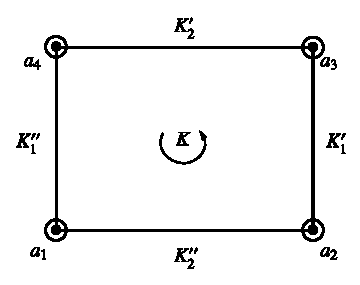
\includegraphics{figure/fig11.2.eps}
\caption{}\label{chap11-fig11.2}
\end{figure}

Splitting the boundary into four parts as in
Fig.~\ref{chap11-fig11.2}, we get
\begin{equation*}
\mathscr{E}_{h}(u,w_{h})=\sum_{K\in\mathfrak{t}_{h}}\left(\Delta_{1,K}\left(u,\frac{\p
  w_{h}}{\p x_{1}}\right)+\Delta_{2,K}\left(u,\frac{\p w_{h}}{\p
  x_{2}}\right)\right),\tag{11.17}\label{chap11-eq11.17} 
\end{equation*}
where for $j=1,2$, we define
\begin{equation*}
\begin{split}
 \Delta_{j,K}\left(u,\frac{\p w_{h}}{\p x_{j}}\right) &=
\int\limits_{K'_{j}}\left(-\Delta u+(1-\sigma)\frac{\p^{2}u}{\p
  \tau^{2}_{K}}\right)\left(\frac{\p w_{h}}{\p
  x_{j}}-\Lambda_{K}\left(\frac{\p w_{h}}{\p
  x_{j}}\right)\right)d\gamma\\
&\quad -\int\limits_{K''_{j}}\left(-\Delta
u+(1-\sigma)\frac{\p^{2}u}{\p \tau^{2}_{K}}\right)\left(\frac{\p
  w_{h}}{\p x_{j}}-\Lambda_{K}\left(\frac{\p w_{h}}{\p
  x_{j}}\right)\right)d\gamma, 
\end{split}\tag{11.18}\label{chap11-eq11.18}
\end{equation*}
$\Lambda_{K}$\pageoriginale being the $Q_{1}$-interpolation operator
associated with the values at the four vertices.

Note that \eqref{chap11-eq11.17} is the same as
\eqref{chap11-eq11.15}. This is evident provided we show that the
contribution of the terms involving $\Lambda_{K}$ is zero. This is so
because $w_{h}=0$ on the boundary $\Gamma$ and on the common
boundaries, $\Lambda_{K}\left(\dfrac{\p w_{h}}{\p x_{j}}\right)$ is
linear and equal in value for both adjacent finite elements since it
agrees at the vertices, but occurs with opposite signs as is obvious
from Fig.~\ref{chap11-fig11.3} $(K^{1'}_{1}=K^{2''}_{1})$.
\begin{figure}[H]
\centering
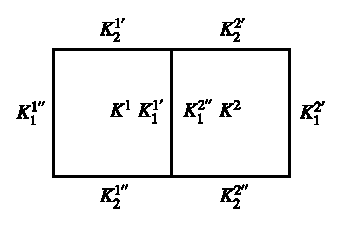
\includegraphics{figure/fig11.3.eps}
\caption{}\label{chap11-fig11.3}
\end{figure}

We also record that $\dfrac{\p w_{h}}{\p
  x_{j}}\Big|_{K}\in\p_{j}P_{K}$ where
\begin{equation*}
\p_{j}P_{K}=\left\{\frac{\p p}{\p x_{j}}:K\to \mathbb{R};\ p\in
P_{K}\right\}.\tag{11.19}\label{chap11-eq11.19} 
\end{equation*}

We now prove a result analogous to the Bramble-Hilbert lemma which
will help us to estimate that $\Delta_{j,K}$'s and hence
$\mathscr{E}_{h}(u,w_{h})$. 

\begin{theorem}[BILINEAR LEMMA]\label{chap11-thm11.2}
Let $\Omega\subset \mathbb{R}^{n}$ be open with Lipschitz continuous
boundary $\Gamma$. Let $W$ be a subspace of $W^{l+1,q}(\Omega)$ such
that $P_{1}\subset W$. Let $b$ be a continuous bilinear form over
$W^{k+1,p}(\Omega)\times W$ such that
$$
\begin{cases}
b(p,w)=0\quad\text{for all}\quad p\in P_{k},\ w\in W\\
b(v,q)=0\quad\text{for all}\quad v\in W^{k+1,p}(\Omega),\ q\in P_{1}. 
\end{cases}
$$

Then\pageoriginale there exists a constant $C=C(\Omega)$ such that for
all $v\in W^{k+1,p}$ $(\Omega)$, $w\in W$,
\begin{equation*}
|b(v,w)|\leq
C||b||~|v|_{k+1,p,\Omega}|w|_{l+1,q,\Omega}.\tag{11.21}\label{chap11-eq11.21} 
\end{equation*}
\end{theorem}

\begin{proof}
For a given $w\in W$, $b(\cdot,w):v\mapsto b(v,w)$ is a continuous
linear form on $W^{k+1,p}(\Omega)$ vanishing on $P_{k}$. Hence by the
Bramble-Hilbert lemma,
\begin{equation*}
|b(v,w)|\leq
C||b(\cdot,w)||^{*}_{k+1,p,\Omega}|v|_{k+1,q,\Omega}.\tag{11.22}\label{chap11-eq11.22} 
\end{equation*}

However for all $q\in P_{1}$, $b(v,w)=b(v,w+q)$ so that
$$
|b(v,w)| \leq ||b||~||v||_{k+1,p,\Omega}||w+q||_{l+1,q,\Omega}
$$
and hence
\begin{align*}
|b(v,w)| &\leq ||b||~||v||_{k+1,p,\Omega}\inf\limits_{q\in
  P_{1}}||w+q||_{l+1,q,\Omega}\\ 
&\leq C||b||~||v||_{k+1,p,\Omega}|w|_{l+1,q,\Omega},\text{~~ by the
  theorem \ref{chap6-thm6.2},}
\end{align*}
so that
$$
||b(\cdot,w)||^{*}_{k+1,p,\Omega}\leq C||b||~|w|_{l+1,q,\Omega}.
$$
and substituting in \eqref{chap11-eq11.22}, we get
\eqref{chap11-eq11.21}, which completes the proof.
\end{proof}

We may now prove the theorem on our error estimate and order of
convergence.

\begin{theorem}\label{chap11-thm11.3}
For a regular family $(\mathfrak{t}_{h})$ of triangulations made up of
Adini's rectangles
\begin{equation*}
||u-u_{h}||_{h}\leq C\ h||u||_{3,\Omega}.\tag{11.23}\label{chap11-eq11.23}
\end{equation*}
\end{theorem}

\begin{proof}
Let us first estimate $|\Delta_{j,K}|$ for $j=1,2$. Set
$$
\begin{cases}
\varphi =-\Delta u+(1-\sigma)\dfrac{\p^{2}u}{\p \tau^{2}_{K}}\in
H^{1}(K),\quad\text{since}\quad u\in H^{3}(\Omega),\\
v=\dfrac{\p w_{h}}{\p x_{1}}\in \p_{1}P_{K}.
\end{cases}
$$

Define\pageoriginale
\begin{equation*}
\delta_{1,K}(\varphi,v)=\int\limits_{K'_{1}}\varphi(v-\Lambda_{K}v)d\gamma-\int\limits_{K''_{1}}\varphi(v-\Lambda_{K}V)d\gamma,\tag{11.24}\label{chap11-eq11.24} 
\end{equation*}
for $v\in\p_{1}P$, $\varphi\in H^{1}(K)$. If $h_{2}$ is the length of
$K'_{1}$ (and $K''_{1}$) and $h_{1}$ is that of $K'_{2}$ (and
$K''_{2}$) we have by a simple change of variable
\begin{equation*}
\delta_{1,K}(\varphi,v)=h_{2}\delta_{1,\hat{K}}(\hat{\varphi},\hat{v}),\tag{11.25}\label{chap11-eq11.25} 
\end{equation*}
where $\hat{K}$ is the reference finite element. Since $P_{0}\subset
Q_{1}$ which is preserved by $\Lambda_{K}$ we have that for all
$\hat{v}\in P_{0}$, $\hat{\varphi}\in H^{1}(\hat{K})$,
$\delta_{1,\hat{K}}(\hat{\varphi},\hat{v})=0$. Now let
$\hat{\varphi}\in P_{0}$ and $\hat{v}\in \widehat{\p_{1}P}$. We wish
to show that $\delta_{1,\hat{K}}(\hat{\varphi},\hat{v})=0$: 

We may take for $\hat{K}$, the unit square. Since $\hat{\varphi}\in
P_{0}$, its value on $\hat{K}$ is a constant, say, $b_{0}$. Now let
$\hat{v}\in \widehat{\p_{1}P}$. Then $\hat{v}$ is of the form
\begin{equation*}
\hat{v}=a_{0}+a_{1}x_{1}+a_{2}x_{2}+a_{3}x^{2}_{1}+a_{4}x_{1}x_{2}+a_{5}x^{2}_{2}+a_{6}x^{2}_{1}x_{2}+a_{7}x^{3}_{2}. \tag{11.26}\label{chap11-eq11.26} 
\end{equation*}

Taking the values at the four vertices we get
\begin{equation*}
\Lambda_{K}\hat{v}=a_{0}+(a_{1}+a_{3})x_{1}+(a_{2}+a_{5}+a_{7})x_{2}+(a_{4}+a_{6})x_{1}x_{2}.\tag{11.27}\label{chap11-eq11.27}
\end{equation*}

Now $K'_{1}$ is the line $x_{1}=1$ and $K''_{1}$ is the line
$x_{1}=0$. Thus
\begin{align*}
&
  \hat{v}-\Lambda_{K}\hat{v}\Big|_{x_{1}=0}=-(a_{5}+a_{7})x_{2}+a_{5}x^{2}_{2}+a_{7}x^{3}_{2},\\
&
  \hat{v}-\Lambda_{K}\hat{v}\Big|_{x_{1}=1}=-(a_{5}+a_{7})x_{2}+a_{5}x^{2}_{2}+a_{7}x^{3}_{2}. 
\end{align*}

Hence,
\begin{equation*}
\begin{split}
\int\limits_{K'_{1}}\hat{\varphi}(\hat{v}-\Lambda_{K}\hat{v})d\gamma
&=
\int\limits^{1}_{0}b_{0}(-(a_{5}+a_{7})x_{2}+a_{5}x^{2}_{2}+a_{7}x^{3}_{2})dx_{2}\\
&=\int\limits_{K''_{1}}\hat{\varphi}(\hat{v}-\Lambda_{K}\hat{v})d\gamma.
\end{split}\tag{11.28}\label{chap11-eq11.28}
\end{equation*}

Thus\pageoriginale $\delta_{1,\hat{K}}(\hat{\varphi},\hat{v})=0$ for
$\hat{\varphi}\in P_{0}$, $\hat{v}\in \widehat{\p_{1}P}$. 

Note further that the bilinear form $\delta_{1,\hat{K}}$ is
continuous, for
\begin{align*}
|\delta_{1,\hat{K}}(\hat{\varphi},\hat{v})| &\leq
C||\hat{\varphi}||_{L^{2}(\p \hat{K})}||\hat{v}||_{L^{2}(\p
  \hat{K})}.\\
&\leq C||\hat{\varphi}||_{1,\hat{K}}||\hat{v}||_{1,\hat{K}},\text{~ by
  the Trace theorem (cf.\@ Th.\@ \ref{chap2-thm2.3}).} 
\end{align*}

Thus we may apply the bilinear lemma to the bilinear form
$\delta_{1,\hat{K}}$ with $l=k=0$ to get
\begin{equation*}
|\delta_{1,\hat{K}}(\hat{\varphi},\hat{v})|\leq
C|\hat{\varphi}|_{1,\hat{K}}|\hat{v}|_{1,\hat{K}}.\tag{11.29}\label{chap11-eq11.29} 
\end{equation*}

We also have the relations
\begin{equation*}
\begin{cases}
|\hat{\varphi}|_{1,\hat{K}}\leq C||B_{K}||~|\det
B_{K}|^{-\frac{1}{2}}|\varphi|_{1,K},\\
|\hat{v}|_{1,\hat{K}}\leq C||B_{K}||~|\det B_{K}|^{-\frac{1}{2}}|v|_{1,K}.
\end{cases}\tag{11.30}\label{chap11-eq11.30} 
\end{equation*}

Now $||B_{K}||\leq C\ h_{K}$ and $|\det B_{K}|=\meas K/\meas
\hat{K}\geq C\rho^{2}_{K}$, and thus $||B_{K}||~|\det
B_{K}|^{-\frac{1}{2}}\leq \dfrac{C\ h_{K}}{\rho_{K}}\leq C$. Also
$h_{2}\leq h_{K}$, so that
\begin{equation*}
|\Delta_{1,K}(\varphi,v)|\leq
C\ h_{K}||u||_{3,K}||w_{h}||_{2,K}\tag{11.31}\label{chap11-eq11.31} 
\end{equation*}
where
$$
\begin{cases}
\varphi=-\Delta u+(1-\sigma)\frac{\p^{2}u}{\p \tau^{2}_{K}},\\
v=\frac{\p w_{h}}{\p x_{1}},
\end{cases}
$$
and similarly,
\begin{equation*}
|\Delta_{2,K}(\varphi,v)|\leq
C\ h_{K}||u||_{3,K}||w_{h}||_{2,K}.\tag{11.32}\label{chap11-eq11.32} 
\end{equation*}

These inequalities lead us to the estimate
\begin{equation*}
|f(w_{h})-a_{h}(u,w_{h})|\leq
Ch||u||_{3,\Omega}||w_{h}||_{h},\tag{11.33}\label{chap11-eq11.33} 
\end{equation*}
for\pageoriginale a {\em regular family} of triangulations made up of
Adini's rectangles. Thus varying $w_{h}$ over $V_{h}$ and taking the
supremum, we get the estimate \eqref{chap11-eq11.11}.

Using \eqref{chap11-eq11.10} and \eqref{chap11-eq11.11} and
substituting in \eqref{chap11-eq11.8} we get the required estimate as
given in \eqref{chap11-eq11.23}. This completes the proof.
\end{proof}

\begin{remark}\label{chap11-rem11.3}
By the Duality Argument, Lesaint and Lascaux \cite{key15} have proved
that $||u-u_{h}||_{1,\Omega}\leq Ch^{2}||u||_{4,\Omega}$ assuming
$u\in H^{4}(\Omega)$. They have also got an improved $0(h^{2})$
convergence order in the $||\cdot ||_{h}$ norm, when all the
rectangles are equal - a ``superconvergence'' result.
\end{remark}

We close this section with a brief description of other types of
finite elements used in non-conforming methods.

\begin{example}\label{chap11-exam11.2}
The Zienkiewicz triangle {\em (cf.\@ Exercise \ref{chap4-exer4.6})}
cf.\@ Fig.~\ref{chap11-fig11.4}.
\begin{figure}[H]
\centering
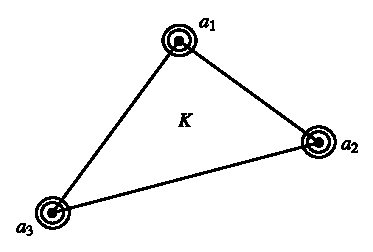
\includegraphics{figure/fig11.4.eps}
\caption{}\label{chap11-fig11.4}
\end{figure}

We get $V_{h}\subset C^{0}(\overline{\Omega})$ only and hence the
method is non-conforming. It does not always yield convergence. The
method works if the sides of all triangles are parallel to three
directions only, as in Fig.~\ref{chap11-fig11.5}.
\begin{figure}[H]
\centering
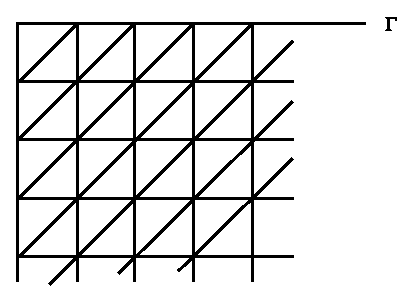
\includegraphics{figure/fig11.5.eps}
\caption{}\label{chap11-fig11.5}
\end{figure}

This\pageoriginale is not so if the number of directions is four, as
in Fig.~\ref{chap11-fig11.6}. (The Union Jack Problem).
\begin{figure}[H]
\centering
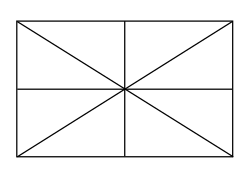
\includegraphics{figure/fig11.6.eps}
\caption{}\label{chap11-fig11.6}
\end{figure}
\end{example}

\begin{example}\label{chap11-exam11.3}
Morley's Triangle (cf.\@ Fig.~\ref{chap11-fig11.7}).
\begin{figure}[H]
\centering
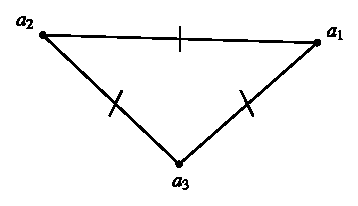
\includegraphics{figure/fig11.7.eps}
\caption{}\label{chap11-fig11.7}
\end{figure}

Here $P_{K}=P_{2}$. We {\em always} get convergence for regular
families, of course. In fact if $u\in H^{4}(\Omega)$, then
\begin{equation*}
||u-u_{h}||_{h}\leq Ch||u||_{4,\Omega}.\tag{11.34}\label{chap11-eq11.34}
\end{equation*}

What is astonishing is that this finite element is not even of class $C^{0}$.
\end{example}

\begin{example}\label{chap11-exam11.4}
{\em Fraeijs de Veubeke triangle.} This finite element is again a
triangle. Apart from the values of the polynomials at the vertices and
the mid-points of the sides, we also take the average normal
derivative along the sides. Here the space $P_{K}$, which we will not
describe, satisfies the inclusion
$$
P_{2}\subset P_{K}\subset P_{3},
$$
and
$$
\sum_{K}=\left\{p(a_{i}),1\leq i\leq 3; p(a_{ij}), 1\leq i<j\leq 3;
\int\limits_{K'_{i}}\frac{\p p}{\p \nu}d\gamma, 1\leq i\leq 3\right\}.
$$

The\pageoriginale finite element is shown symbolically in
Fig.~\ref{chap11-fig11.8}. 
\begin{figure}[H]
\centering
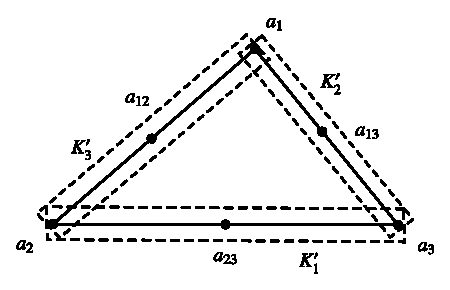
\includegraphics{figure/fig11.8.eps}
\caption{}\label{chap11-fig11.8}
\end{figure}

Here also the finite element is not of class $C^{0}$ in general, but
the method always yields convergence.
\end{example}

\noindent
{\bf References:}~For general reference on non-conforming methods, see\break Strang and Fix \cite{key22}, for the bilinear lemma, see Ciarlet
\cite{key29}. For a detailed study of the Zienkiewicz triangle,
Moreley's triangle and Fraeijs de Veubeke triangle, see Lascaux and
Lesaint \cite{key15}. For a nonconforming method with penalty, see
Babuska and Zl\'amal \cite{key26}.

\begin{thebibliography}{99}
\bibitem{key1} BRAMBLE,\pageoriginale J.H: THOM\'EE, V.

Interior maximum norm estimates for some simple finite element
methods. {\em Revue Fran\c{C}aise d'Automatique, Informatique,
  Recherche Operationelle} (RAIRO), R-2, (1974), pp.-5-18.

\bibitem{key2} BRAMBLE, J.H; ZL\'AMAL, M.

Triangular elements in the finite element methods, {\em Mathematics of
  Computation}, 24, (1970), pp.~809-820.

\bibitem{key3} BREZIS, H; STAMPACCHIA, G.

Sur la r\'egularit\'e de la solution d'in\'equations elliptiques, {\em
  Bull. Soc. Math. France}, 96(1968), pp.~153-180.

\bibitem{key4} CIARLET, P.G.

Sur l'\'el\'ement de Clough et Tocher, {\em RAIRO}, R-2, (1974),
pp.~19-27. 

\bibitem{key5} CIARLET, P.G; RAVIART, P.-A.

{\em La M\'ethodes des \'El\'ements Finis pour les Probl\`ems aux
  Limites Elliptiques}, (to appear).

\bibitem{key6} CIARLET, P.G; RAVIART, P.-A.

Maximum principle and uniform convergence for the finite element
method, Computer Methods in Applied Mechanics and Engineering, 2,
(1973), pp.~17-31.

\bibitem{key7} CIARLET, P.G; RAVIART, P.-A.

General Lagrange and Hermite interpolation in $\mathbb{R}^{n}$ with
applications to finite element methods, {\em Arch. Rational
  Mech. Anal.} 46, (1972), pp.~177-199.

\bibitem{key8} CIARLET, P.G; WAGSCHAL, C.

Multipoint Taylor formulas and applications to the finite element
method, {\em Numer. Math.,} 17, (1971), pp.~84-100.

\bibitem{key9} CIAVALDINI, J.F; NEDELEC, J.C.

Sur l'\'el\'ement de Fraeijs de Veubeke et Sander, {\em RAIRO}, R-2,
(1974), pp.~29-45.

\bibitem{key10} DUVAUT, G; LIONS, J.-L.

{\em Les In\'equations en M\'ecanique et en Physique}, Dunod, Paris (1972).

\bibitem{key11} FALK, R.S.

Error estimates for the approximation of a class of variational
inequalities, {\em Math. Comput}. (to appear).

\bibitem{key12} FALK, R.S.\pageoriginale

Approximation of an elliptic boundary value problem with unilateral
constraints, {\em RAIRO}, (to appear).

\bibitem{key13} HABER, S.

Numerical evaluation of multiple integrals, {\em SIAM Review}, 12,
(1970), pp.~481-526.

\bibitem{key14} LANDAU, L; LIFCHITZ, E.

{\em Th\'eorie de l'Elasticit\'e}, Mir, Moscow (1967).

\bibitem{key15} LASCAUX, P; LESAINT, P.

Some non-conforming finite elements for the plate bending problem,
{\em RAIRO}, (to appear).

\bibitem{key16} LEWY, H; STAMPACCHIA, G.

On the regularity of the solution of a variational inequality, {\em
  Comm. Pure Appl. Math.,} 22, (1969), pp.~153-188.

\bibitem{key17} LIONS, J.-L; MAGENES, E.

{\em Probl\`emes aux Limites non Homogenes et Applications.} Vol.~1,
Dunod, Paris, (1968).

\bibitem{key18} LIONS, J.-L; STAMPACCHIA, G.

Variational inequalities, {\em Comm. Pure Appl. Math.,} 20,
(1967). pp.~493-519. 

\bibitem{key19} MOSCO, U; STRANG, G.

One-sided approximation and variational inequalities, {\em
  Bull. Amer. Math. Soc.} 80 (1974), pp.~308-312.

\bibitem{key20} NE\v{C}AS, J.

{\em Les M\'ethodes Directes en Theorie des Equations Elliptiques,}
Masson, Paris, (1967).

\bibitem{key21} STRANG, G.

Approximation in the finite element method, {\em Number. Math.,}
19(1972), pp.~81-98.

\bibitem{key22} STRANG, G; FIX, G.J.

{\em An Analysis of the Finite Element Method}, Prentice-Hall,
Englewood Cliffs, (1973).

\bibitem{key23} \v{Z}ENI\v{S}EK, A.

Interpolation polynomials on the triangle, {\em Numer. Math.,} 15,
(1970), pp.~283-296.

\bibitem{key24} \v{Z}ENI\v{S}EK, A.

Polynomial approximation on tetrahedrons in the finite element method,
{\em J. Approximation Theory}, 7, (1973), pp.~334-351.

\bibitem{key25} ZL\'AMAL, M.\pageoriginale

On the finite element method, {\em Numer. Math.,} 12, (1968), pp.~394-409.

\bibitem{key26} BABU\v{S}KA, I.; ZL\'AMAL, M.

Nonconforming elements in the finite element method with penalty, {\em
  SIAM J. Numer. Anal.,} 10(1973), pp.~863-875.

\bibitem{key27} BRAMBLE, J.H.; HILBERT, S.R.

Estimation of linear functionals on Sobolev spaces with application to
Fourier transforms and spline interpolation, {\em SIAM
  J. Numer. Anal.,} 7, (1970), pp.~113-124.

\bibitem{key28} BRAMBLE, J.H.; HILBERT, S.R.

Bounds for a class of linear functionals with applications to Hermite
interpolation, {\em Numer. Math.,} 16, (1971), pp.~362-369.

\bibitem{key29} CIARLET, P.G.

Conforming and nonconforming finite element methods for solving the
plate problem, in {\em Conference on the Numerical Solution of
  Differential Equations} (G.A. WATSON, Editor), pp.~21-31, Lecture
Notes in Mathematics, Vol.~363, Springer-Verlag, Berlin (1974).

\bibitem{key30} CIARLET, P.G.; RAVIART, P.-A.

Interpolation theory over curved elements, with applications to finite
element methods, {\em Comp. Methods in Appl. Mech. and Engineering,}
1, (1972), pp.~217-249.

\bibitem{key31} CIARLET, P.G.; RAVIART, P.-A.

The combined effect of curved boundaries and numerical integration in
isoparametric finite element methods, in {\em The Mathematical
  Foundations of the Finite Element Method with Applications to
  Partial Differential Equations} (A.K. AZIZ, Editor), pp.~409-474,
Academic Press, New York, (1972).

\bibitem{key32} ZL\'AMAL, M.

A finite element procedure of the second order of accuracy, {\em
  Numer. Math.,} 16, (1970), pp.~394-402.
\end{thebibliography}

\newpage

\begin{center}
{\Large\bf Additional References}\pageoriginale
\end{center}

\noindent
{\bf Books} (Additional References)

\begin{description}
\item[BABUSKA, I; AZIZ, A.K.] First part of `{\em The Mathematical
  Foundations of the Finite Element Method with applications to
  Partial Differential Equatios}' (Symposium, University of Maryland,
  Baltimore, June-26-30, 1972) (Edited by A.K. AZIZ) Academic\break Press,
  New York, (1972).

\item[NORRIE, D.H; DE VRIES, G.] {\em The Finite Element Method -
  Fundamentals and Applications}, Academic Press, New York, (1973).

\item[ODEN, J.T.] {\em Finite Elements of Nonlinear Continue}, McGraw
  Hill,\break  New York, (1972).

\item[ZIENKIEWICZ, O.C.] {\em The finite Element Method in Engineering
  Science}, McGraw Hill, London, (1971).
\end{description}

{\em Journals} (where articles dealing with the finite element method
may be regularly found).

Revue Fran\c{c}aise d'Automatique, Informatique, Recherche
Operationelle (RAIRO), ``Red'' Series

Computer Methods in Applied Mechanics and Engineering.

International Journal for Numerical Methods in Engineering.

Mathematics of Computation.

SIAM Journal on Numerical Analysis

Numerische Mathematik.

{\em Proceedings of Conferences totally or partially devoted to the
  finite element method:}

{\em The Mathematics of Finite Elements and Applications},
(Conference, Brunel University, 18-20 April, 1972), Edited by
J.R. WHITEMAN, Academic Press, London, 1973.

{\em Conference on the Numerical Solution of Differential Equations},
(Conference, Dundee, 03-06 July 1973), Edited by G.A. WATSON, Lecture
Notes in Mathematics, Vol. {\em 363}, Springer-Verlag, New York, 1974.

{\em The\pageoriginale Mathematical Foundations of the Finite Element
  Method with Applications to Partial Differential Equations|,
  (Symposium, University of Maryland, Baltimore, 26-30 June. 1972),
  Edited by A.K. AZIA, Academic Press. New York, 1972.

{\em Computing Methods in Applied Science and Engineering}, Vol. 1 and
2 (International Symposium IRIA LABORIA, Versailles, 17-21 December,
1973) Edited by R. GLOWINSKI and J.L. LIONS, Lecture notes in Computer
Science, Vol., {\em 10} and {\em 11}, Springer-Verlag, New York, 1974.

{\em Topics in Numerical Analysis} (Royal Irish Academy Conference on
Numerical Analysis, Dublin, 1972), Edited by J.J.H. MILLER, Academic
Press, New York, 1973.

{\em Mathematical Aspects of Finite Elements in Partial Differential\break
  Equations} (Symposium, 01-03 April, 1974, Mathematics Research
Center, The University of Wisconsin, Madison), Edited by C. de BOOR,
Academic Press, New York, 1974.

Proceedings of the {\em Second Conference on the Mathematics of Finite
  Elements and Applications}, (Brunel University, April 07-10, 1975,
to appear.) 
